\chapter{~}
Friday morning, I woke up around 7:00 am. I wanted to get ready for the drive to Cincinnati,
so I got out the truck, and went to fill the tanks with gas. I also checked the oil and tire
pressure. As I was doing this, I noticed that the sky was somewhat dark off to the west. I was
hoping that we wouldn't get a lot of rain. After I had finished, I returned home, but I didn't
put the truck back in the garage, I just pulled behind the gate, and parked it under the oak
tree, since we'd be leaving before long.

I went inside, grabbed a quick shower, and started to lay out the materials we'd use for
the casts I would put on Monique. I hoped her ankle was better, but it really wouldn't hurt us
if it wasn't. I would put the long leg cast on her left leg, so she wouldn't be bearing any
weight on it if she crutched. We would take the wheelchair also, just in case. I thought of
loading the wheelchair up now, but decided not to, just in case I wanted to use it to get her to
the truck.

At about 8:00, it started raining. Not good. By 8:30, I was hearing thunder. Even worse. I
turned on the television, looking for a weather report. They were predicting storms for the
whole area today. I began to consider alternate plans. Perhaps we could go somewhere and public
indoors, such as a museum or mall. As I considered ideas, Monique knocked on the door.

I opened the door to Monique looking very nice, holding an umbrella.

``Hi, Quinn,'' she said. ``Nice day to walk around outside, huh?''

``Beautiful day for it,'' I responded sarcastically. I noticed that the rain had picked up
a bit. ``Come on inside, we'll figure out what we're going to do.''

She came in, and we sat down in the parlor. I noticed that she was walking well, with no
trace of a limp. ``How's the ankle?'' I asked her.

``It's fine. It wasn't a very bad sprain, really.'' She lied.

``Good.''

``So- what are we going to do?''

``I don't know. Publicking outside is out. You can't hold an umbrella while using crutches
or a wheelchair, and the drowned rat look takes a lot away from the glamour.''

Monique was disappointed; she'd really been looking forward to it. I went on: ``We have
two options, as I see it. We can go someplace and do it indoors, or we could stay here and do a
session- maybe with some more adventuresome casting.''

\begin{thought}
``More adventuresome casting'' Monique thought to herself. That sounds interesting. I
wonder what he means.
\end{thought}

``The weather isn't great for a lot of driving, either,'' Monique said. ``What do you mean
by more adventuresome casting?''

Recalling the thoughts I'd had after casting Samantha on Wednesday, I said ``Something
bigger than what you've done before.''

Monique was excited, but hid it well. ``How big?'' She asked.

I drew my breath, then said ``A body cast. A body cast that covers your torso, one arm and
one leg. If you're up for it.''

\begin{thought}
Wow! A hip spica/shoulder spica combination! She was excited about the prospect, but
didn't want to show it. It would be great to be in that cast. She wouldn't be able to do much,
but the sensations should be awesome!
\end{thought}

``Wow, that would be big,'' she said. She didn't sound too negative as she said it, which
I hoped was a good sign. She stood up and walked to the window, and looked outside. ``I think
that would be better than going out in this weather. It looks like the rain is picking up.'' As
if to punctuate her comment, thunder rolled off in the distance. ``Let's go for it,'' she
finished.

I was thrilled at the prospect, but tried to hide it. ``Well, I need to make a few
preparations,'' I said. ``I had things set up for the leg casts.'' I stood up and walked to the
casting room, and she followed. In the casting room, I opened the closet, and got out some more
fiberglass.

``Is there anything I can do to help?'' She asked, surprising me.

``No, not really- I just need to get out more materials,'' I said, taking out more
padding, and also getting out the roll of twelve inch stockinette.

With the materials laid out, I picked up the bucket.

``Monique, I'll go fill this. I'll need you to strip down to your bra and underwear.''

``OK,'' she said, curling up one leg and slipping off her sandal as I left.

\begin{thought}
Monique couldn't believe this was going to happen. Looking around online at pictures,
stories and anecdotes about casting, she'd learned about many different types of casts, and some
had definitely appealed to her as ones she wanted to wear. The shoulder/hip spica combo was one
that had she had really liked the idea of wearing, and today she was going to get to wear one!
She wondered a bit about his telling her to leave her bra on. Was he going to make the cast
cover both shoulders, or did he intend to leave the bra strap showing? Maybe he wanted to slip
the strap off of that shoulder and hide it under the cast. She hoped that wasn't the case, as it
would probably be uncomfortable. As she finished undressing, she wished she'd known that this
was going to happen today- she'd have worn a strapless bra if she'd only known.
\end{thought}

When I returned to the casting room, Monique was folding up her clothes and putting them
on the chair. She looked incredible, with her tanned skin contrasting with the black lingerie
she wore. I put the bucket on the cart as she sat on the casting table. I turned to her and
talked about how we would go about making the cast.

``Monique, this cast will be huge, and tricky to make. We'll make it from the top down. If
things get too uncomfortable at any time, let me know, and we'll change the plan or stop. I
don't want this to be painful for you.''

``I'll be fine,'' she said. ``I'm getting used to this, and I know by now that you're
considerate and careful not to hurt me.''

I felt good, hearing her say that. I took a lot of care to make things as comfortable as
possible for the models. ``I think I want a cigarette before we start. How about you?''

``Yes, I do, too.'' She said. I took my pack, and offered her one. I lit it for her, and
then one for myself.

``Are we going to use plaster or fiberglass?'' she asked.

``Fiberglass,'' I answered. ``A plaster cast that big would take 24 hours to dry and I
don't think you want to be stuck that way for nearly that long.''

``No, that wouldn't be too much fun,'' she lied. \aside{Actually, I think it WOULD be fun,
she thought to herself.}

I cut off a four foot long piece of the twelve inch stockinette, and turned to her. I
asked her to stand up and raise her arms. When she did, I slid the stockinette over her head,
and pulled it down past her hips. I took my scissors, and made vertical cuts upward at the
armpits, allowing the stockinette to fall down in a front and rear flap. I had her lower her
arms, and then took the flaps and raised them to cover the upper parts of her chest and back. I
taped the two flaps together over each shoulder. As I started cutting off a piece of three inch
stockinette for her arm, she stopped me with a question.

``Is the cast going to cover both of my shoulders?

``No, only the left one. We'll leave the right one bare.''

``Do you want my bra strap to show?''

``Not really, but there really isn't much of a choice.''

Monique steeled herself for what she'd planned to do next. ``How about this?'' She asked
as she pulled the stockinette up from the bottom, slid her arms underneath it behind her, and
unfastened her bra. She then brought her arms around front and pulled it off. She brought out
her arms, tossed her bra into the chair, and pulled the stockinette back down to below her butt
and smoothed it out. Outside, another round of thunder sounded. It was still in the distance,
but was louder than before. She turned to me, face slightly red, and asked ``Is that better?''

I was absolutely stunned. I couldn't help but look at how her breasts pressed outward
against the tight stockinette. ``Yes, it's better. Are you sure you want to do it this way?''

Monique blushed a bit further as she said ``If we're going to do this, we might as well do
it right. Just don't ask me to take off any more.''

``Monique, I would never have asked you to do what you just did!''

``I know that. If you had asked, I probably would have walked out. But, you have shown me
that you are very professional. I'm OK with this.''

I didn't know what to say, so I just went back to making the cast. I slid the stockinette
over her left arm, all the way to the part already covering her body. I made a slit for her
thumb and pulled it through. I then cut a length of four inch stockinette for her leg. I had her
sit down on a stool, and I put it on her leg all the way to the top of the thigh. I moved her
long dark hair to the right side, letting it drape over the right shoulder, out of the way. I
then began wrapping padding on her arm, starting at the armpit, and working down to the hand. I
then took some six inch padding, and began wrapping at her hips, working my way upward over her
chest, shoulder and upper arm.

We were both more comfortable with the padding on her chest, but I did miss the view.
Despite my opinions about her, Monique was extremely beautiful. I could never deny having
enjoyed seeing her with just the stockinette on her chest, which was not much different than
seeing her totally topless. I pulled on a pair of gloves, and got the broom handle from the
corner. I handed the broom handle to her, and she took it in her left hand. I positioned her arm
the way I wanted, and asked her to hold it that way and sit up straight while I put the
fiberglass on. I also instructed her to take full breaths as I wrapped the casting tape over her
chest, so that she'd be able to breathe easily when the cast was dry. I tore open a roll of five
inch white fiberglass, and started wrapping on her upper arm, working over the shoulder and
downward. I stopped the downward progress before I got to where the padding ended. I was careful
not to smash her chest. I used several more rolls to give the thickness needed, and then started
just above the elbow, working downward to the wrist. When the desired thickness had been reached
there, I clipped off the flap over her right shoulder, and folded down the edges of stockinette
and padding around the area where her head and right arm came through the cast. I used another
roll of five inch white fiberglass to anchor it, making sure to get the tape to lay smooth.

The surface of the fiberglass on her arm was sweating out droplets of water as it dried. I
decided that it was set enough to hold her arm in place, so I took the broom handle from her,
and placed it back in the corner. I finished the cast over her hand, and after it had been
folded over and anchored, I decided it was time for a break. I took off the gloves and tossed
them.

``Are you OK, Monique?''

\begin{thought}
Am I OK?! I am fantastic! She thought to herself. She had enjoyed every turn of the
fiberglass as she felt its weight being wrapped around her body. As Quinn applied the cast, she
enjoyed how it played to her senses; watching his hands work quickly, yet carefully, the fruity
smell of the wet fiberglass, but most of all, the sensation of being encased. That was exciting
her intensely. The thunderstorm brewing outside made the whole experience even more surreal. She
felt the heat of a blush in her face, and hoped he would take is as a reaction to the setting
fiberglass, which was quite warm. She had enjoyed every cast he had put on her, but this one put
all of the others to shame. The feeling of the fiberglass as he wrapped it over her breasts was
almost too much to bear. She wanted to give in totally to the feelings, but knew she could not.
Still, enjoying it in silence seemed only to heighten the experience for her. Finally, she
answered him.
\end{thought}

``I'm fine,'' She said. ``It's a bit warm, but not too bad.'' Outside, the thunder clapped
again. ``It's a good thing we stayed here,'' she went on. ``That storm is getting closer.''

``It is.''

``I love a good thunderstorm,'' she said. ``I love the sounds and smells of a storm.''

``As long as they don't get too strong,'' I replied.

``True.''

We chatted a few minutes longer while we waited for the fiberglass to dry. When it was, I
had her stand up. I had her bend over and lean against the wall with her uncasted arm. I wanted
to cast her in a seated position, and this seemed to be the best way to get the angle I wanted
from her hip. I checked with her to make sure she was comfortable in that position, and then
started wrapping more padding where I had left off. When the padding was wrapped all the way
down to her ankle, I tore open another roll of five inch fiberglass, and started wrapping at the
waist, working downward.

\begin{thought}
Monique struggled to keep her knees from shaking as she felt layer after layer of
fiberglass being wrapped around her waist and hips. As he continued down her thigh, she hoped he
wouldn't be able to notice her excitement at the feelings it was giving her. Roll after roll,
down her thigh, over her slightly bent knee, down to her ankle. She was enjoying this in a way
she'd never experienced enjoyment before. Although she knew it would, she didn't want it to end.
She wanted to tell Quinn the truth about enjoying it right then and there, but knew that it
would cause serious awkwardness. She also feared that it would make him decide to end the
adventure right there. He might even decide not to work with her again. She wished he could
enjoy this as much as she did.
\end{thought}

As I worked on casting Monique's hip and leg, I marveled at what I was actually doing.
Just six months before, casting a beautiful woman was only a dream, and now it was happening. As
I made each turn with the fiberglass, making sure it lay smoothly; I couldn't help but dream
further. As great as this was, how much better if the woman I were casting actually enjoyed it.
I was happy to be doing it the way I was, but it would be the ultimate to cast a woman who did
it for fun, rather than did it for money.

``How are you doing? Still OK?'' I asked her.

``Yes, I'm still good,'' she said.

I went about carefully anchoring the stockinette and padding in the areas I had just
wrapped. I had to be very careful to not touch her inappropriately. I pulled back the
stockinette, and made slits to allow it to fold over the edges of the fiberglass without
bunching. I used a final roll in the area to hold down these edges, and when it was done, I was
very pleased with the way it turned out.

\begin{thought}
As Quinn trimmed up the stockinette around her most sensual areas, Monique once again was
tortured trying to conceal her enjoyment. He was very careful not to touch her in any way
remotely unprofessional. She could sense his hands passing close, but the mostly set fiberglass
prevented her from actually feeling him. She longed to feel his hands at that moment. As the
thunder got louder and louder outside, she was thankful for the storm, and for this wonderful
experience it had afforded her. After he finished that area, he helped her stand up, away from
the wall. He held her up, as she was unable to balance herself. She was taking in the
experience, being moved around with her back, hip, leg and arm held tightly by the cast.
\end{thought}

Almost finished, I stood Monique up, and let her lean back into my arms. I stooped a bit,
and picked her up. Although she was heavy with her new fiberglass clothes, I was able to pick
her up and place her on the casting table. She took her right arm and placed it behind her to
keep from falling over onto her back. It didn't take long for me to wrap padding and fiberglass
around her foot. I stood back and took in the entire cast, and it was impressive. She was
covered with smooth white fiberglass. Only her neck, head, right leg, and right shoulder and arm
were uncovered. She looked unbelievable.

``How does the cast feel?'' I asked her. ``Are you comfortable?''

``It feels fine,'' she said. \aside{It feels a lot better than fine, she thought to
herself. I wish I could tell you how great it feels.}

She looked so beautiful in the cast that I decided to do a sketch of her right there.

``Monique, I think I want to do a sketch right now. We'll probably do another one later,
but I'd like to capture you on paper just as you sit.''

``That's fine with me,'' she answered cheerfully.

I retrieved my pad and pencils, sat down across from her, and started to work. I was
amazed at the way the pencil moved across the paper. She almost seemed to jump onto the page.

\begin{thought}
As Quinn drew, Monique was enjoying the cast. She was enjoying the way it held her snugly.
She tried moving against the cast in various areas. She tried moving her leg, then her hips,
followed by her back and shoulder. She was vaguely aware of the sounds of the storm outside, but
she was thoroughly distracted by the feelings of the cast- there was almost no moving against
it. It wasn't tight, yet it was very snug. She could take a deep, full breath, but that was all
the slack there was in the cast. She was also totally engrossed in watching Quinn draw. It
reminded her slightly of watching her father paint when she was young. She enjoyed watching both
of them work.
\end{thought}

When the sketch was done, I showed it to Monique.

``Wow, I had an image in my mind of what I must look like in this cast, but it's still
surprising to see it on paper. This is really a huge cast.''

``Yes, it's a monster. Let's go to the other room and get some pictures.''

``Okay.''

I wheeled her into the parlor, and noticed something I'd missed. The casting room had
blinds, which were kept drawn for obvious reasons. When we were in the parlor, I looked out the
window, and it looked nearly like night outside. The storm was on us. The wind was blowing, and
the thunder was louder and more often. I'd been so wrapped up in making the cast that I really
hadn't noticed how loud it was getting.

``Wow, it's really dark out there. This is more than a little rain,'' I said.

``It really is. I hope it doesn't get nasty.'' She said, thinking to herself how she had
missed the storms strengthening during the process of getting the cast.

I got my camera out, and started taking pictures of Monique in the wheelchair from various
angles. I used up a whole roll of 36 exposures before I knew it. I picked her up and set her on
the couch, and as I reloaded the camera, I noticed the sky outside starting to lighten up a
little bit.

I worked my way thought the next roll of film, and was nearly done when I heard a sound
that snapped me to reality very quickly- The long wail of the civil defense siren. I looked out
the window again, and noticed that the sky had a serious green tint to it. That was very bad.
Tornado sky. I noticed that the lightning flashes and thunderclaps were almost simultaneous-
close strikes. I turned on the television. The weather was already on. The meteorologist said we
were under a tornado warning- there had been several touchdowns to the west of us, and it was
going to be on us within minutes. We had to take shelter immediately!

``Monique, we have to get to the basement!''

``I can't get there on my own!''

But, before she had gotten the words out, I was already behind her, pushing the chair
toward the kitchen. I stopped in the kitchen and got the flashlight out of the drawer, and
grabbed my battery powered boom box from the closet. I pushed her around the corner, and leaned
the chair back as I carefully lowered the chair down the steps, one at a time. The steps were
barely wide enough to get her down, with her arm out to the side as it was. Outside, the wind
was howling, the thunder was incredibly loud and frequent, and underneath it all was the
constant keening wail of the siren.

Once we had reached the bottom of the stairs, I turned her chair into the main room, and
turned on the light.

``Are you OK?'' I asked her.

``Yes, I think so. It's really getting bad up there.''

``Yes it is. I'm glad we didn't go out. We'd have been on the road in this,'' I said.

``It's a good thing you had the idea to stay in,'' she commented.

``A better idea would have been to check the weather report before I put you in such a
big $\ldots$'' My words were cut off by the loudest crack of thunder I'd ever heard, followed
by a huge crashing sound. The light went out.

``Oh shit,'' Monique murmured.

I said ``That's putting it mildly'' as I turned on the radio, and then the flashlight. The
radio station had people out in the town, giving on the spot reports on what they were seeing:
``… reports on the police scanner of three different tornadoes on the ground…. BILL, I''VE GOT
TO GET TO COVER! I CAN SEE A TORNADO ON THE GROUND FROM WHERE I AM!!!''

I could hear a distant roaring sound. It sounded like a train, just as you hear so many
tornado survivors speaking of. I looked at Monique, and I saw fear in her eyes. The radio was
still going- the people in the station were seeking shelter, but promising to stay on the air.
Their words were as if in a dream- I was listening to the sounds outside. I could hear the
roaring, the wind, and the sound of things hitting the house. I realized it must be hail. Dear
God, the tornado was going to hit us!

\newpage
\begin{center}
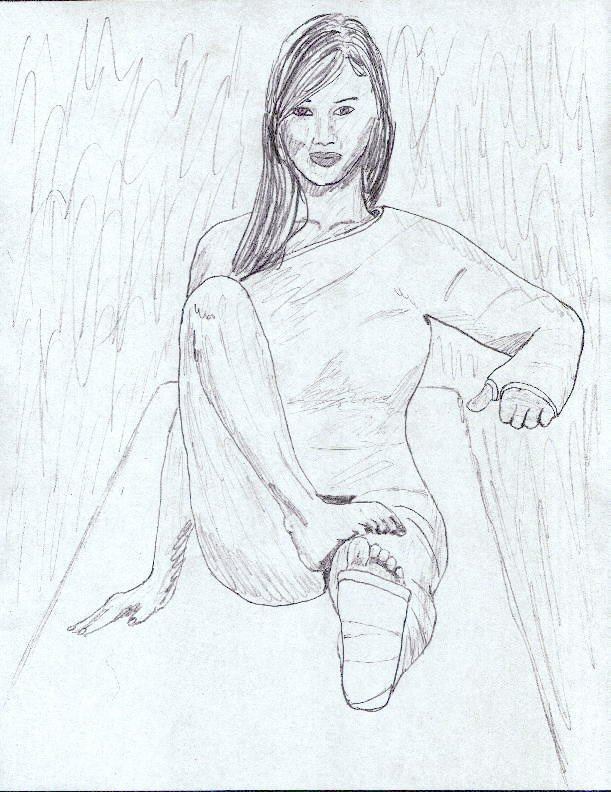
\includegraphics{images/kicks26.jpg}
\end{center}
